\message{ !name(11-16_seconddertest.tex)}\documentclass[11pt,reqno,final]{amsart}

\pdfcompresslevel=0
\pdfobjcompresslevel=0

\usepackage[dvipsnames]{xcolor}% adds colors
\usepackage{amsmath, amsthm}% {amsfonts, amssymb}

% New Characters
\usepackage[latin1]{inputenc}%
\usepackage[T1]{fontenc}

\usepackage{MnSymbol}
\usepackage[normalem]{ulem}% underlining

\usepackage[theoremfont, largesc]{newpxtext} % different text,math font
\usepackage{newpxmath}

\makeatletter
\DeclareMathRadical{\sqrtsign}{symbols}{112}{largesymbols}{112}
% \let\sqrt=\undefined
% \DeclareRobustCommand\sqrt{\@ifnextchar[\@sqrt{\mathpalette\@x@sqrt}]}
% \def\@x@sqrt#1#2{%
%  \setbox\z@\hbox{$\m@th#1\sqrtsign{\mkern1mu #2}$}
%  \mkern3mu\box\z@}
\makeatother




% Page Typesetting
\usepackage[final]{microtype}
\usepackage{relsize}
\usepackage[margin=1in]{geometry}
\usepackage{framed}
\usepackage{tikz}

\usepackage{csquotes}

\usepackage{setspace}
\onehalfspacing

\usepackage{hyperref}
\hypersetup{
  final,
  pdftitle={Math 135 - Second Derivative Test},
  pdfauthor={Bonventre}, 
  linktoc=page,
  pagebackref,
  colorlinks=true,
  citecolor=PineGreen,
  linkcolor=PineGreen,
  linkbordercolor=PineGreen,
}


% Internal References

\usepackage[inline,shortlabels]{enumitem}

% \numberwithin{equation}{section} 
\numberwithin{figure}{section}

\usepackage[nameinlink,capitalise,noabbrev]{cleveref}

\crefname{equation}{}{} % get \cref to behave as \eqref

% \theoremstyle{plain} % bold name, italic text
\newtheorem{theorem}[equation]{Theorem}%
\newtheorem*{theorem*}{Theorem}%
\newtheorem{lemma}[equation]{Lemma}%
\newtheorem{proposition}[equation]{Proposition}%
\newtheorem{corollary}[equation]{Corollary}%
\newtheorem{conjecture}[equation]{Conjecture}%
\newtheorem*{conjecture*}{Conjecture}%
\newtheorem{claim}[equation]{Claim}%
\newtheorem{question}{Question}

\theoremstyle{definition} % bold name, plain text
\newtheorem{definition}[equation]{Definition}%
\newtheorem*{definition*}{Definition}%
\newtheorem{example}[equation]{Example}%
\newtheorem*{example*}{Example}%
\newtheorem{remark}[equation]{Remark}%
\newtheorem{notation}[equation]{Notation}%
\newtheorem{convention}[equation]{Convention}%
\newtheorem{assumption}[equation]{Assumption}%
\newtheorem{exercise}[question]{Exercise}

% ---------- macros
\newcommand{\set}[1]{\left\{#1\right\}}%
\newcommand{\sets}[2]{\left\{ #1 \;|\; #2\right\}}%
\newcommand{\longto}{\longrightarrow}%
\newcommand{\into}{\hookrightarrow}%
\newcommand{\onto}{\twoheadrightarrow}%

\usepackage{harpoon}
\newcommand{\vect}[1]{\text{\overrightharp{\ensuremath{#1}}}}

\newcommand{\del}{\partial}%

\newcommand{\ki}{\chi}
\newcommand{\ksi}{\xi}
\newcommand{\Ksi}{\Xi}

\newcommand{\dlim}{\displaystyle\lim}

% %%%%%%%%%%%%%%%%%%%%%%%%%%%%%%%%%%%%%%%%%%%%%%%%%%%%%%%%%%%%%%%%%%%%%%%%%%%%%%%%%%%%%%%%%%%%%%%%%%%%

\begin{document}

\message{ !name(11-16_seconddertest.tex) !offset(20) }
{Concavity}

The first derivative says whether the original function $f(x)$ is \textbf{increasing} or \textbf{decreasing}.
The second derivative talks about the \textit{curvature}, in particular the \textbf{concavity}, of the graph.

\begin{framed}
        \begin{gather*}
                \mbox{$f''(x) > 0$ for $x \in (a,b)$
                  $\Rightarrow$
                  $f$ is \textbf{concave up} on $(a,b)$
                  $\Rightarrow$
                  the \textit{slope} is \textbf{increasing} on $(a,b)$
                }\\
                \mbox{$f''(x) < 0$ for $x \in (a,b)$
                  $\Rightarrow$
                  $f$ is \textbf{concave down} on $(a,b)$
                  $\Rightarrow$
                  the \textit{slope} is \textbf{decreasing} on $(a,b)$
                }
        \end{gather*}
\end{framed}
\begin{center}
        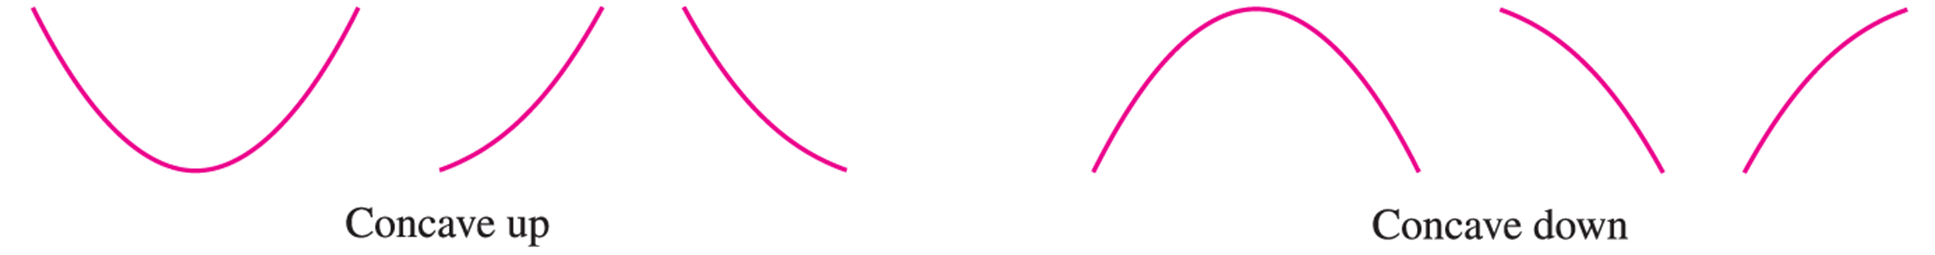
\includegraphics[width=\textwidth]{11-16P_concave}
\end{center}

An \textbf{inflection point} $x = c$ is a point where the concavity \textit{changes}:
\begin{itemize}
\item $f''(c) = 0$, and
\item the sign of $f''$ flipes on either side of $x = c$.
\end{itemize}
\subsection*{Warning.} An \textit{inflection point} corresponds to the notion of a \textit{local extremum}, \textbf{not} a critical point!

\begin{example}
        Together, let's find teh inflection points of the function $f(x) = (x-2)^3$.
        We will also find the intervals where $f$ is concave up and down.
        \vfill
\end{example}


\section{Second Derivative Test}

The second derivative can also be used to classify critical points:
\subsection*{Second Derivative Test}
Suppose that $x = c$ is a critical point of $f$.
\message{ !name(11-16_seconddertest.tex) !offset(20) }

\end{document}
